%
% sep.tex -- QAM decodierbarkeit
%
% (c) 2020 Prof Dr Andreas Müller, Hochschule Rapperswil
%
\documentclass[tikz,12pt]{standalone}
\usepackage{times}
\usepackage{amsmath}
\usepackage{txfonts}
\usepackage[utf8]{inputenc}
\usepackage{graphics}
\usepackage{color}
\usepackage{pifont}
\usetikzlibrary{arrows,intersections,math,calc}
\begin{document}

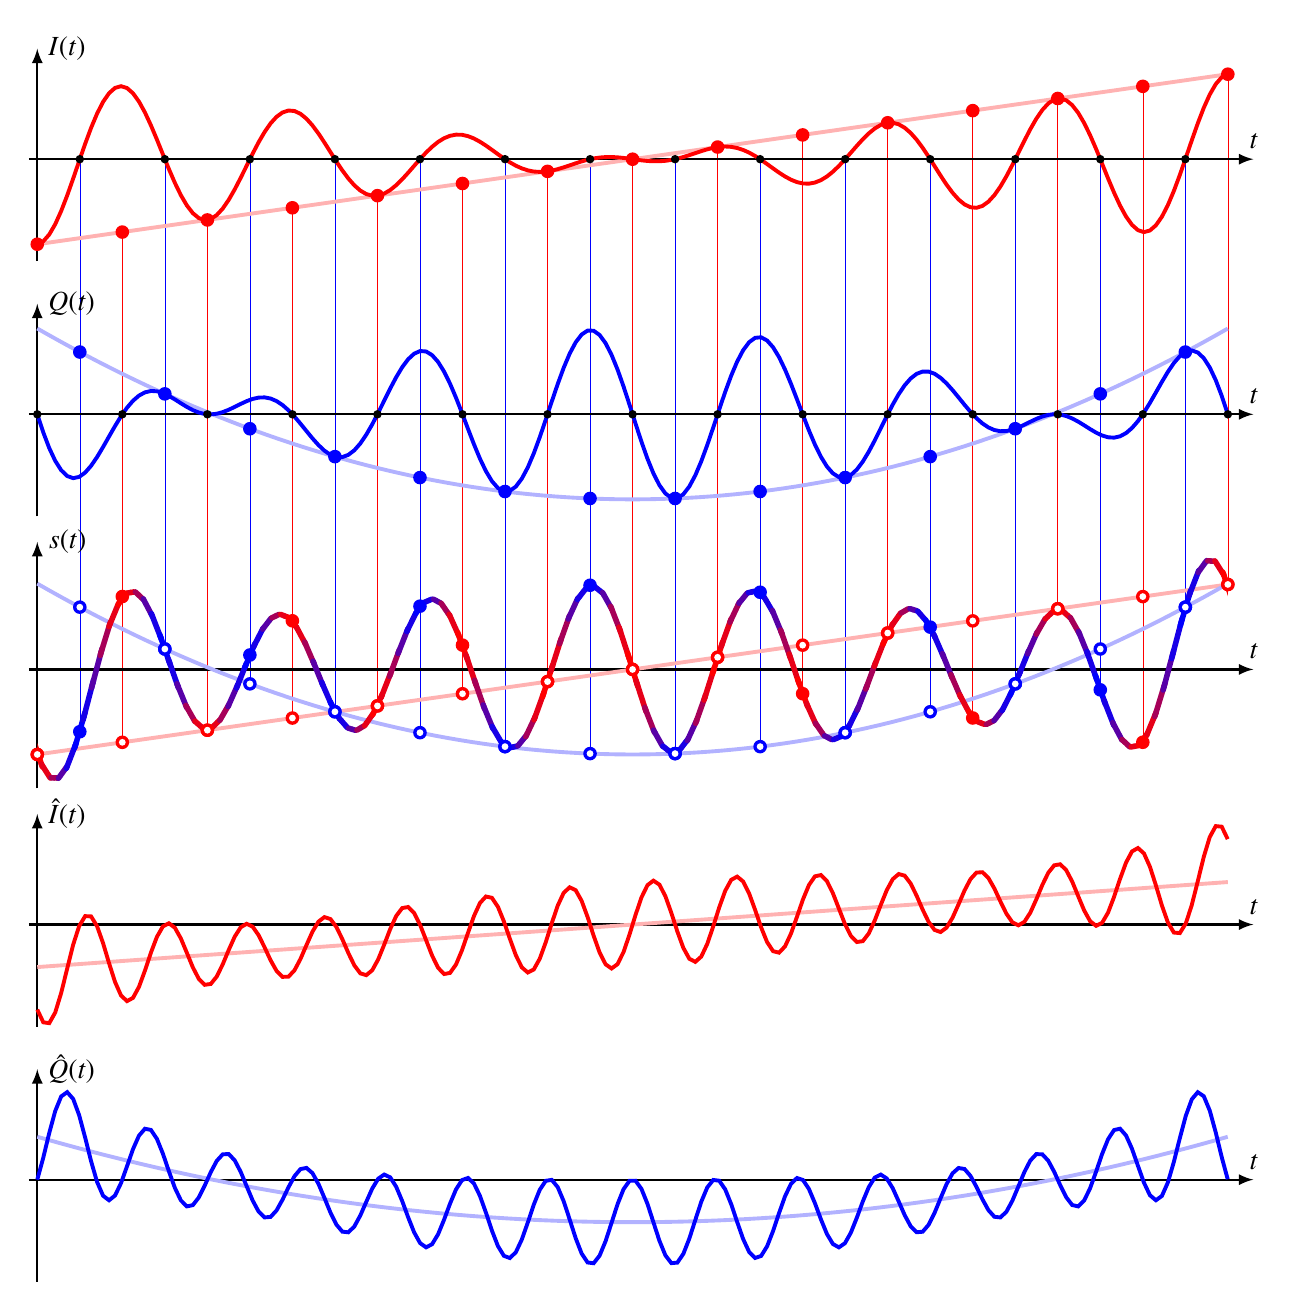
\begin{tikzpicture}[>=latex,thick,scale=1.08]

\def\a{0.1428}
\def\b{-1.0}
\def\c{1}
\def\d{0.041}
\def\o{180}

\begin{scope}[yshift=-6cm]
	\foreach \x in {1,...,14}{
		\pgfmathparse{(\a*\x+\b)*cos(\x*\o)-(\d*(\x-7)*(\x-7)-\c)*sin(\x*\o)}
		\xdef\y{\pgfmathresult}
		\pgfmathparse{\a*\x+\b}
		\xdef\yu{\pgfmathresult}
		\draw[color=red,line width=0.2pt]
			({\x},{min(\y,\yu)}) -- ({\x},{\yu+6});
	}

	\foreach \x in {0.5,1.5,...,14}{
		\pgfmathparse{(\a*\x+\b)*cos(\x*\o)-(\d*(\x-7)*(\x-7)-\c)*sin(\x*\o)}
		\xdef\y{\pgfmathresult}
		\pgfmathparse{\d*(\x-7)*(\x-7)-\c}
		\xdef\yu{\pgfmathresult}
		\draw[color=blue,line width=0.2pt]
			({\x},{min(\y,\yu)}) -- ({\x},{6});
	}
\end{scope}

%
% Graph für I(t) mit Modulation
%
\begin{scope}
	\draw[->] (-0.1,0) -- (14.3,0) coordinate[label={$t$}];
	\draw[->] (0,-1.2) -- (0,1.3) coordinate[label={right:$I(t)$}];
	\draw[color=red!30,line width=1.4pt] plot[domain=0:14,samples=3]
		({\x},{\a*\x+\b});
	\draw[color=red,line width=1.4pt] plot[domain=0:14,samples=200]
		({\x},{(\a*\x+\b)*cos(\x*\o)});
\end{scope}

%
% Graph für Q(t) mit Modulation
%
\begin{scope}[yshift=-3cm]
	\draw[->] (-0.1,0) -- (14.3,0) coordinate[label={$t$}];
	\draw[->] (0,-1.2) -- (0,1.3) coordinate[label={right:$Q(t)$}];
	\draw[color=blue!30,line width=1.4pt] plot[domain=0:14,samples=100]
		({\x},{\d*(\x-7)*(\x-7)-\c});
	\draw[color=blue,line width=1.4pt] plot[domain=0:14,samples=200]
		({\x},{-(\d*(\x-7)*(\x-7)-\c)*sin(\x*\o)});
\end{scope}

%
% Decodierung des modulierten Signals
%
\begin{scope}[yshift=-6cm]
	\draw[->] (-0.1,0) -- (14.3,0) coordinate[label={$t$}];
	\draw[->] (0,-1.4) -- (0,1.5) coordinate[label={right:$s(t)$}];
	\draw[color=red!30,line width=1.4pt] plot[domain=0:14,samples=3]
		({\x},{\a*\x+\b});
	\draw[color=blue!30,line width=1.4pt] plot[domain=0:14,samples=100]
		({\x},{\d*(\x-7)*(\x-7)-\c});


	\begin{scope}
		\def\deltax{0.1}
		\clip (0,-1.4) rectangle (14,1.4);
		\foreach \x in {0,\deltax,...,14.1}{
			\pgfmathparse{cos(\o*\x)*cos(\o*\x)}
			\xdef\rot{\pgfmathresult}
			\pgfmathparse{sin(\o*\x)*sin(\o*\x)}
			\xdef\blau{\pgfmathresult}
			\definecolor{farbe}{rgb}{\rot,0,\blau}
			\pgfmathparse{\x-0.7*\deltax}
			\xdef\xleft{\pgfmathresult}
			\pgfmathparse{(\a*\xleft+\b)*cos(\xleft*\o)-(\d*(\xleft-7)*(\xleft-7)-\c)*sin(\xleft*\o)} 
			\xdef\yleft{\pgfmathresult}
			\pgfmathparse{\x+0.7*\deltax}
			\xdef\xright{\pgfmathresult}
			\pgfmathparse{(\a*\xright+\b)*cos(\xright*\o)-(\d*(\xright-7)*(\xright-7)-\c)*sin(\xright*\o)}
			\xdef\yright{\pgfmathresult}
			\draw[round cap-round cap,color=farbe,line width=2pt]
			({\xleft},{\yleft})
			--
			({\xright},{\yright});
		}
	\end{scope}

	\foreach \x in {0,1,...,14}{
		\pgfmathparse{(\a*\x+\b)*cos(\x*\o)-(\d*(\x-7)*(\x-7)-\c)*sin(\x*\o)}
		\xdef\y{\pgfmathresult}
		\fill[color=red] ({\x},{\y}) circle[radius=0.08];
		\fill[color=red] ({\x},{\y*cos(\x*\o)}) circle[radius=0.08];
		\fill[color=white] ({\x},{\y*cos(\x*\o)}) circle[radius=0.04];
		\fill[color=red] ({\x},{6+\y*cos(\x*\o)}) circle[radius=0.08];
		\fill[color=black]
			({\x},3) circle[radius=0.05];
	}

	\foreach \x in {0.5,1.5,...,14}{
		\pgfmathparse{(\a*\x+\b)*cos(\x*\o)-(\d*(\x-7)*(\x-7)-\c)*sin(\x*\o)}
		\xdef\y{\pgfmathresult}
		\fill[color=blue] ({\x},{\y})
			circle[radius=0.08];
		\fill[color=blue] ({\x},{\y*(-sin(\x*\o))})
			circle[radius=0.08];
		\fill[color=white] ({\x},{\y*(-sin(\x*\o))})
			circle[radius=0.04];
		\fill[color=blue] ({\x},{3+\y*(-sin(\x*\o))})
			circle[radius=0.08];
		\fill[color=black] ({\x},6)
			circle[radius=0.05];
	}

\end{scope}

\begin{scope}[yshift=-9cm]
	\draw[->] (-0.1,0) -- (14.3,0) coordinate[label={$t$}];
	\draw[->] (0,-1.2) -- (0,1.3) coordinate[label={right:$\hat{I}(t)$}];
	\draw[color=red!30,line width=1.4pt] plot[domain=0:14,samples=3]
		({\x},{0.5*(\a*\x+\b)});
	\draw[color=red,line width=1.4pt] plot[domain=0:14,samples=200]
		({\x},{((\a*\x+\b)*cos(\x*\o)-(\d*(\x-7)*(\x-7)-\c)*sin(\x*\o))*cos(\x*\o)});

\end{scope}

\begin{scope}[yshift=-12cm]
	\draw[->] (-0.1,0) -- (14.3,0) coordinate[label={$t$}];
	\draw[->] (0,-1.2) -- (0,1.3) coordinate[label={right:$\hat{Q}(t)$}];
	\draw[color=blue!30,line width=1.4pt] plot[domain=0:14,samples=100]
		({\x},{0.5*(\d*(\x-7)*(\x-7)-\c)});
	\draw[color=blue,line width=1.4pt] plot[domain=0:14,samples=200]
		({\x},{((\a*\x+\b)*cos(\x*\o)-(\d*(\x-7)*(\x-7)-\c)*sin(\x*\o))*(-sin(\x*\o))});

\end{scope}

\end{tikzpicture}

\end{document}

